\anexo{Resultados de la encuesta}

La encuesta fue realizada a un total de 159 personas, superando el mínimo de 120 encuestados para garantizar representatividad. A continuación se presentan las capturas de Google Forms con la distribución de respuestas.

\begin{figure}[!htbp]
  \centering
  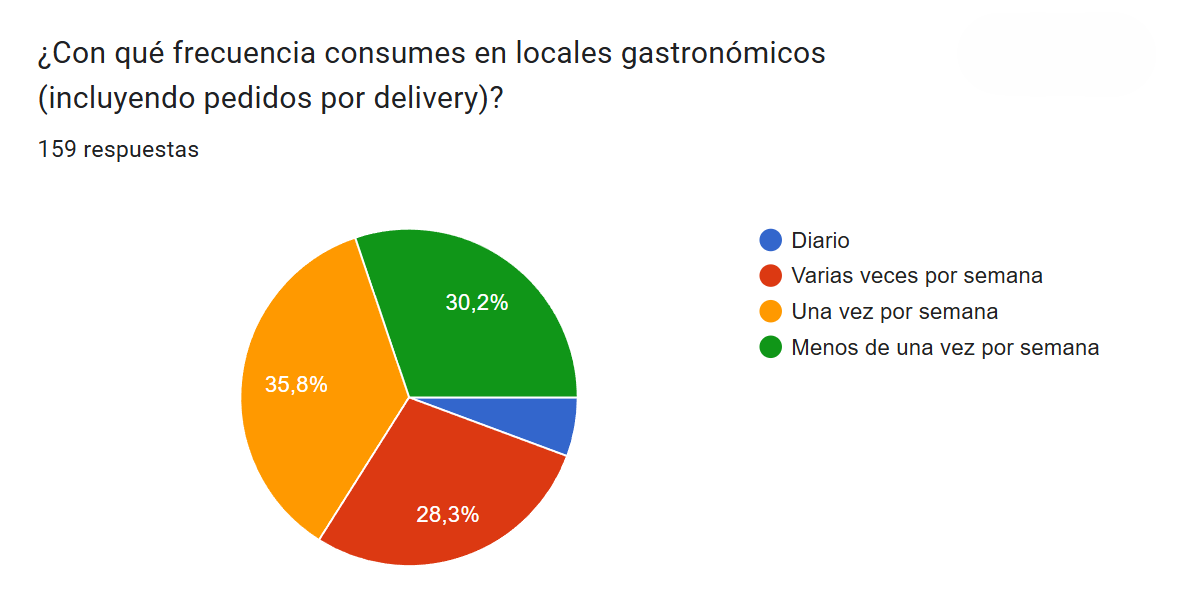
\includegraphics[width=0.75\textwidth]{images/pregunta1.png}
  \caption{¿Con qué frecuencia consumes en locales gastronómicos (incluyendo pedidos por delivery)?}
  \label{fig:anexo-p1}
\end{figure}

\begin{figure}[!htbp]
  \centering
  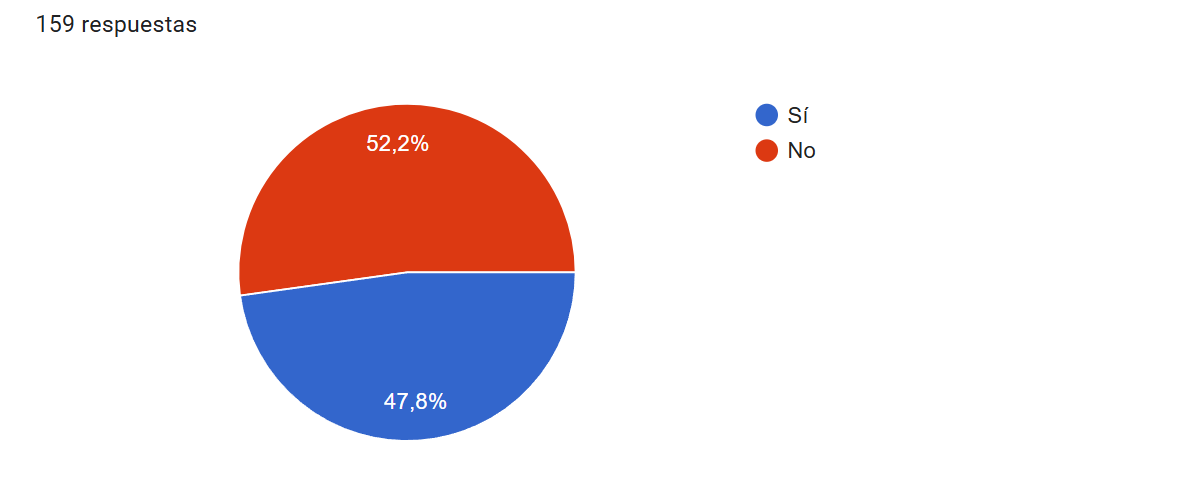
\includegraphics[width=0.75\textwidth]{images/pregunta2.png}
  \caption{¿En el último mes te pasó que el plato o producto que querías pedir no estaba disponible?}
  \label{fig:anexo-p2}
\end{figure}

\begin{figure}[!htbp]
  \centering
  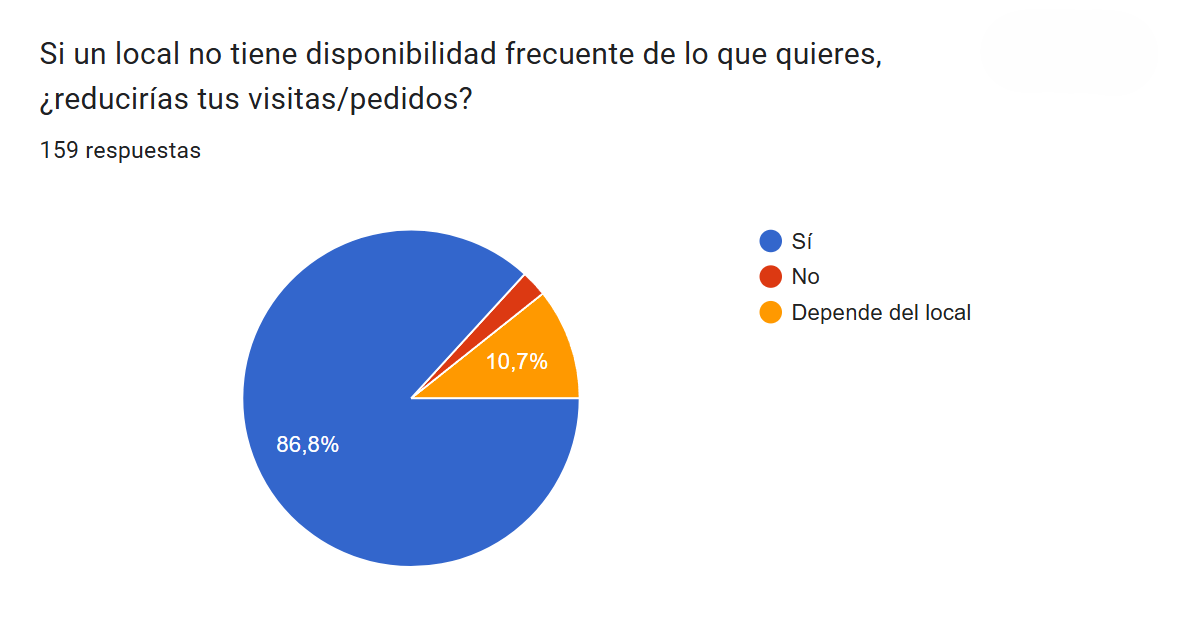
\includegraphics[width=0.75\textwidth]{images/pregunta3.png}
  \caption{Si un local no tiene disponibilidad frecuente de lo que quieres, ¿reducirías tus visitas/pedidos?}
  \label{fig:anexo-p3}
\end{figure}

\begin{figure}[!htbp]
  \centering
  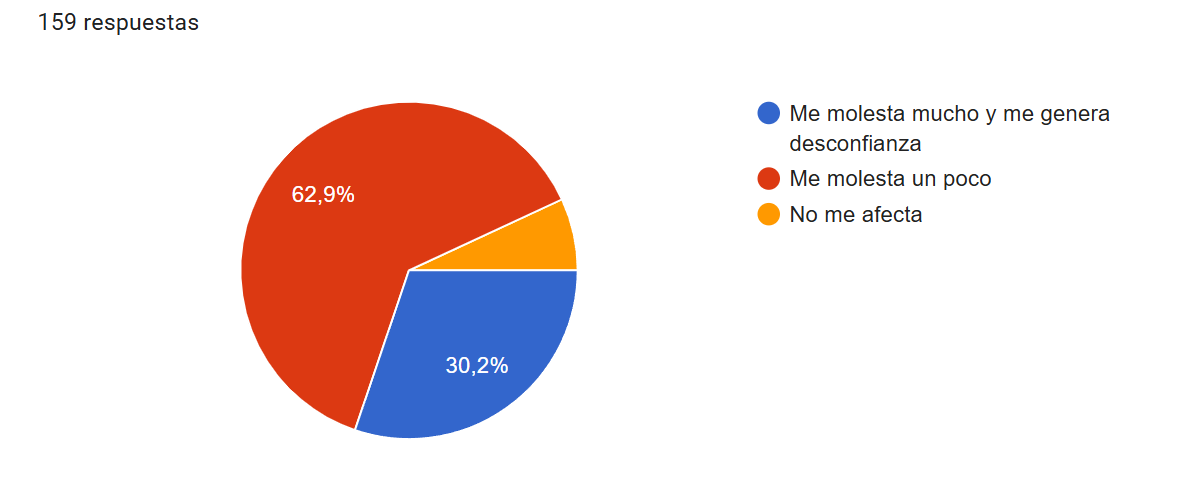
\includegraphics[width=0.75\textwidth]{images/pregunta4.png}
  \caption{¿Cómo afecta en tu percepción que un local no tenga disponibles los platos anunciados en su menú?}
  \label{fig:anexo-p4}
\end{figure}

\begin{figure}[!htbp]
  \centering
  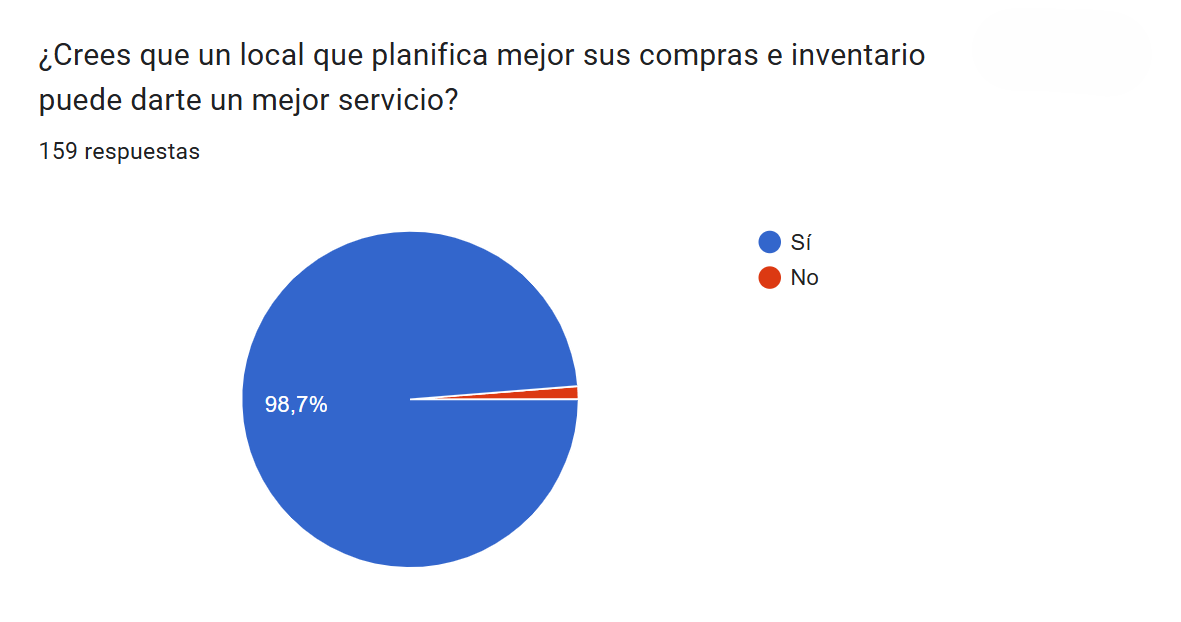
\includegraphics[width=0.75\textwidth]{images/pregunta5.png}
  \caption{¿Crees que un local que planifica mejor sus compras e inventario puede darte un mejor servicio?}
  \label{fig:anexo-p5}
\end{figure}

\begin{figure}[!htbp]
  \centering
  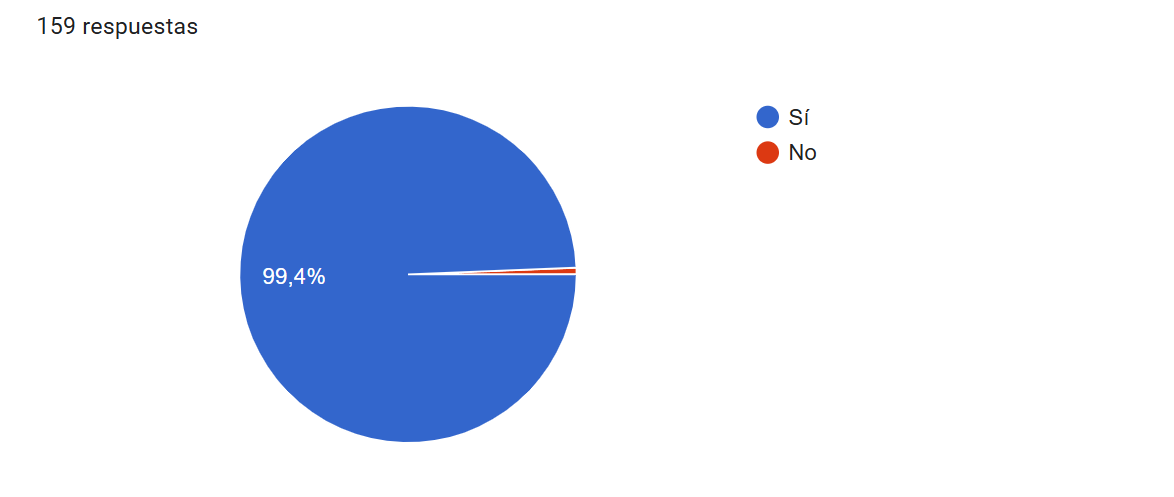
\includegraphics[width=0.75\textwidth]{images/pregunta6.png}
  \caption{Si un local mantiene siempre su menú disponible y con la misma calidad, ¿es más probable que vuelvas?}
  \label{fig:anexo-p6}
\end{figure}

\begin{figure}[!htbp]
  \centering
  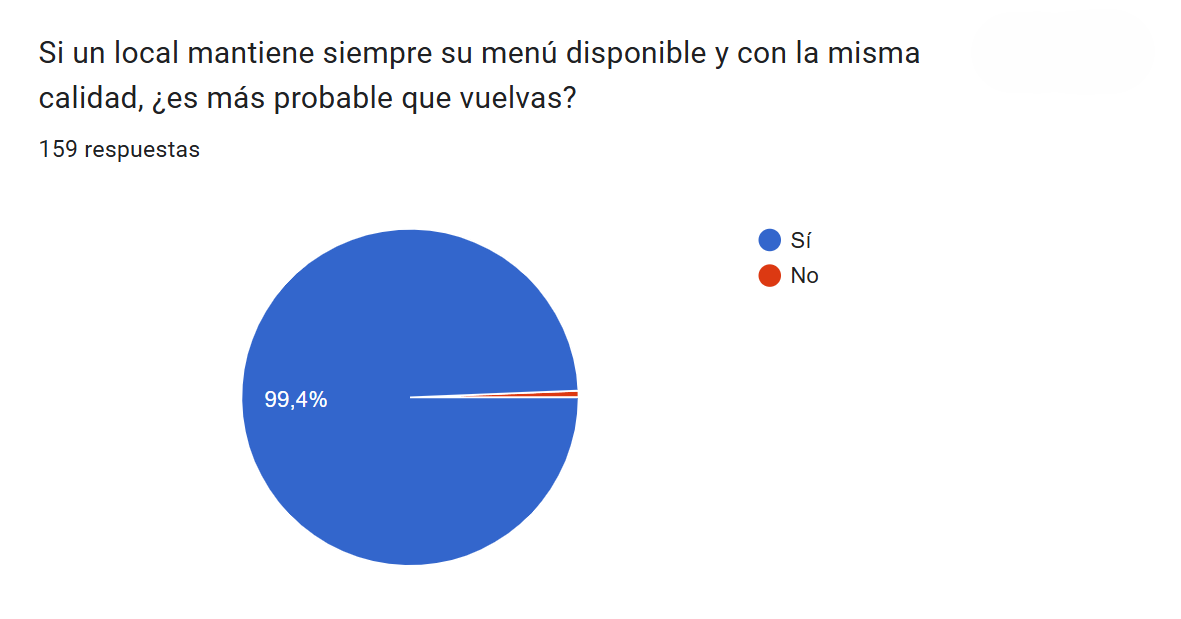
\includegraphics[width=0.75\textwidth]{images/pregunta7.png}
  \caption{¿Recomendarías más un local que siempre tiene disponible los productos que ofrece?}
  \label{fig:anexo-p7}
\end{figure}

\begin{figure}[!htbp]
  \centering
  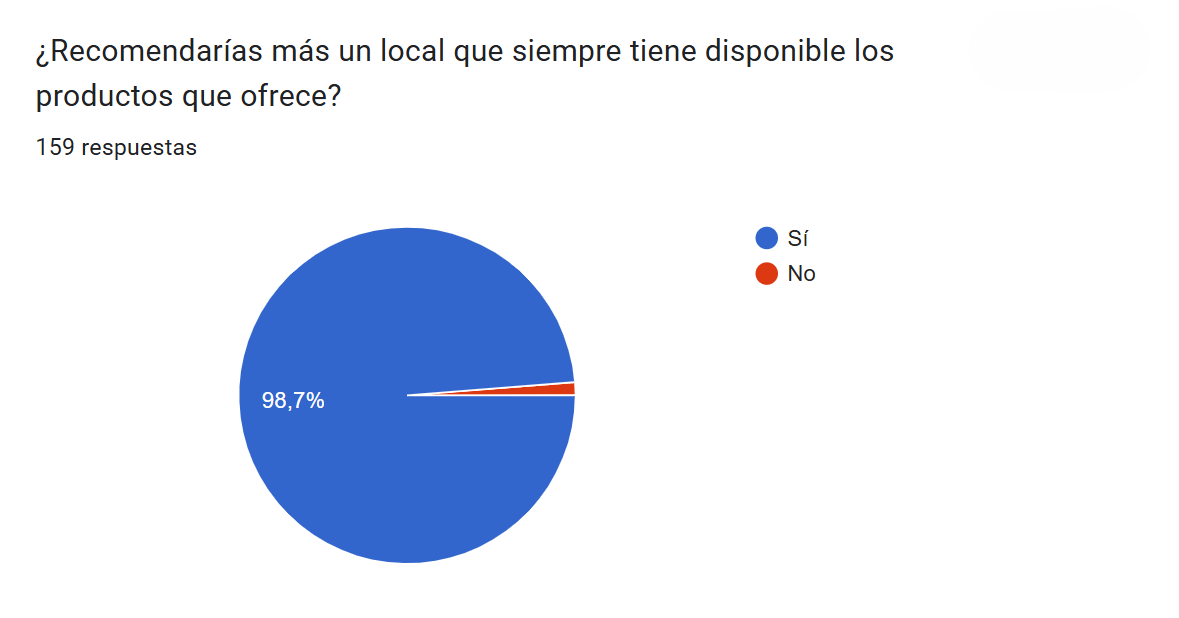
\includegraphics[width=0.75\textwidth]{images/pregunta8.png}
  \caption{¿Consideras que la falta frecuente de platos afecta la reputación del local?}
  \label{fig:anexo-p8}
\end{figure}

% Opcional, para forzar que todo lo anterior se coloque antes de seguir:
\FloatBarrier
